\documentclass[11pt]{beamer}
\usepackage{graphicx}
\usepackage{cancel}	%para cancelar expresiones en fórmulas
\usepackage{multicol}
\usepackage{multirow}
\usepackage{amsmath}
\usepackage{float}
\usepackage{url}
\usepackage{color}
\usepackage{tablefootnote}
\usepackage[12pt]{moresize}	%más tamaños de letra
\usepackage{bm}	%bold para math

\usepackage{titlesec}
%\titleformat{\chapter}[display]
%{\normalfont\bfseries}{}{12pt}{\Huge}	%quitar header de chapter

\usepackage{siunitx}	%support for units, numbers
\sisetup{output-decimal-marker={.}, separate-uncertainty}

\usepackage{hyperref}
\hypersetup{
	colorlinks=true,
	linkcolor=blue,
	citecolor=red,
	bookmarksopen=true,
	bookmarksopenlevel=1,
	urlcolor=blue
}

\usepackage{tikz}	%%TIKZ for drawings, shapes
\usetikzlibrary{positioning}
\tikzset{
	nodo/.style={
		rectangle,
		draw,
		black,
		thick,
		rounded corners,
		node distance=1.5cm,
		inner sep=0.3cm,
		font=\large
	}
}

%%% NOMBRES DE COSAS
\renewcommand{\abstractname}{Abstract}
\renewcommand{\figurename}{Figure}
\renewcommand{\tablename}{Table}
\renewcommand{\contentsname}{Table of Contents}
\renewcommand{\appendixname}{Appendix}
\renewcommand{\bibname}{References}
\renewcommand{\chaptername}{Chapter}

%%% COMANDOS COMUNES
\newcommand{\dif}{\text{d}}
\newcommand{\ddt}[1]{\frac{\dif #1}{\dif t}}
\newcommand{\der}[2]{\frac{\dif #1}{\dif #2}}
\newcommand{\mder}[3]{\frac{\dif^{#3}#1}{\dif #2^{#3}}}		%derivada múltiple
\newcommand{\norm}[1]{\left\| #1 \right\|}
\newcommand{\an}{($\alpha$,n) }
\newcommand{\Aliso}{\textsuperscript{27}Al }
\newcommand{\Piso}{\textsuperscript{30}P }
\newcommand{\Na}{\textsuperscript{22}Na }

%%%%%%%%%%%%%%%%%%%%%%%%%%%%%%%%%%%%%%%%%%%%%%%
\usetheme{Boadilla}
\setbeamercovered{transparent} 
\setbeamertemplate{navigation symbols}{} 
\makeatother
\setbeamertemplate{footline}{
	\leavevmode
	\hbox{
		\begin{beamercolorbox}[wd=.4\paperwidth,ht=2.25ex,dp=1ex,center]{author in head/foot}
			\usebeamerfont{author in head/foot}\insertshortauthor
		\end{beamercolorbox}
		\begin{beamercolorbox}[wd=.6\paperwidth,ht=2.25ex,dp=1ex,center]{title in head/foot}
			\usebeamerfont{title in head/foot}\insertshorttitle\hspace*{3em}
			\insertframenumber{} / \inserttotalframenumber\hspace*{1ex}
		\end{beamercolorbox}
	}
	\vskip0pt
}
\makeatletter

\author{Erik Cárdenas Mayoral}
\title{Measurement of \an reactions in CNA/HiSPANoS}
\titlegraphic{
\includegraphics[scale=0.075]{us.png}} 
\institute{Inter-University Master's Degree in Nuclear Physics}
\date{28/02/2024} 


\begin{document}

\begin{frame}
\titlepage
\end{frame}

%\begin{frame}
%\tableofcontents
%\end{frame}

\begin{frame}{Introduction}
	\[ ^\text{A}_\text{Z}\text{X} + ^4_2\text{He}^{2+} \longrightarrow \text{ } ^{\text{A}+3}_{\text{Z}+2}\text{Y} + \text{n}     \]
	\begin{figure}[H]
		\centering
		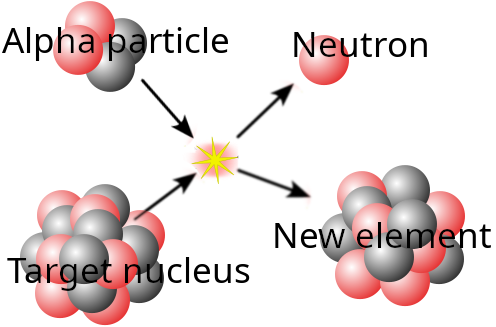
\includegraphics[width=0.45\textwidth]{anreaction.png}
		\caption{Illustration of an \an reaction.}
		\label{anreaction}
	\end{figure}
\end{frame}

\begin{frame}{Relevance of \an reactions}
	\begin{itemize}
		\item Underground particle physics experiments: neutron background
		\item 4 to \qty{9}{\MeV} $\alpha$ particles
	\end{itemize}
	\begin{figure}[H]
		\centering
		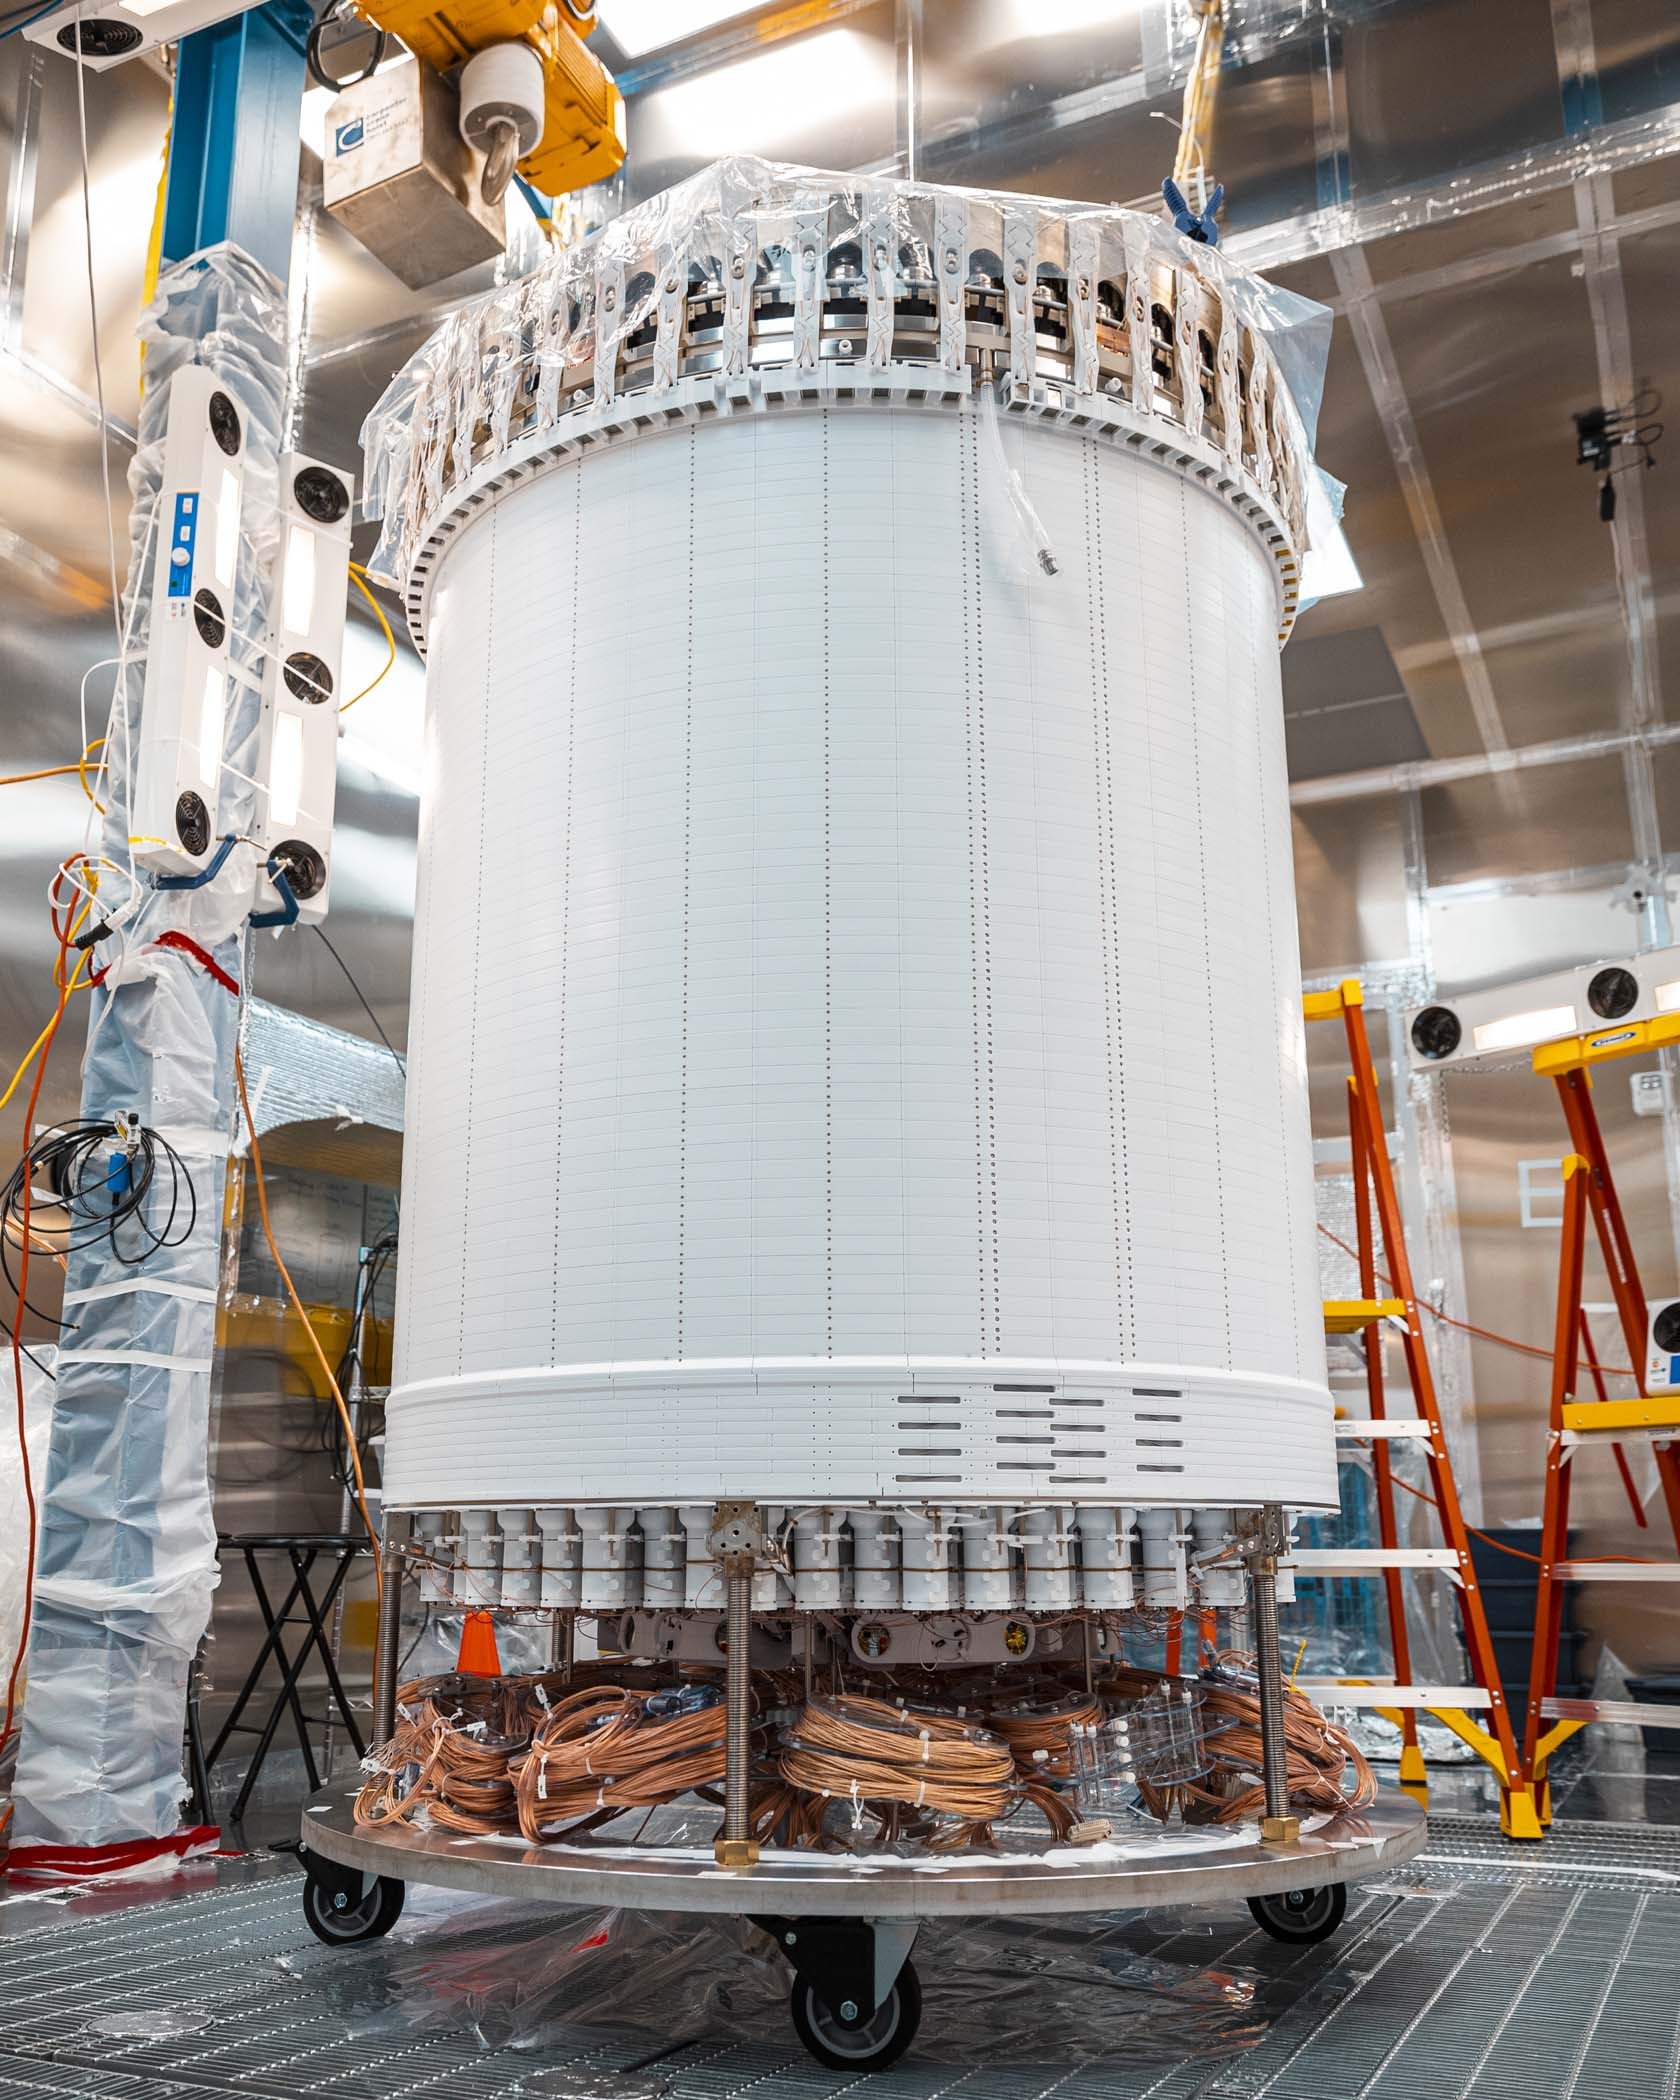
\includegraphics[width=0.35\textwidth]{sanford.jpg}
		\caption{LUX-ZEPLIN experiment, \qty{1.5}{\kilo\meter} deep. Source: \href{https://sanfordlab.org/experiment/lux-zeplin}{sanfordlab.org}}
		\label{}
	\end{figure}
\end{frame}

\begin{frame}{Objective of the thesis}
	\begin{itemize}
		\item Study the viability of \an measurements at CNA/HiSPANoS
		\item To that end, carry out TTY (activation) and energy spectra (ToF) measurements of \Aliso\an
	\end{itemize}
	\begin{figure}[H]
		\centering
		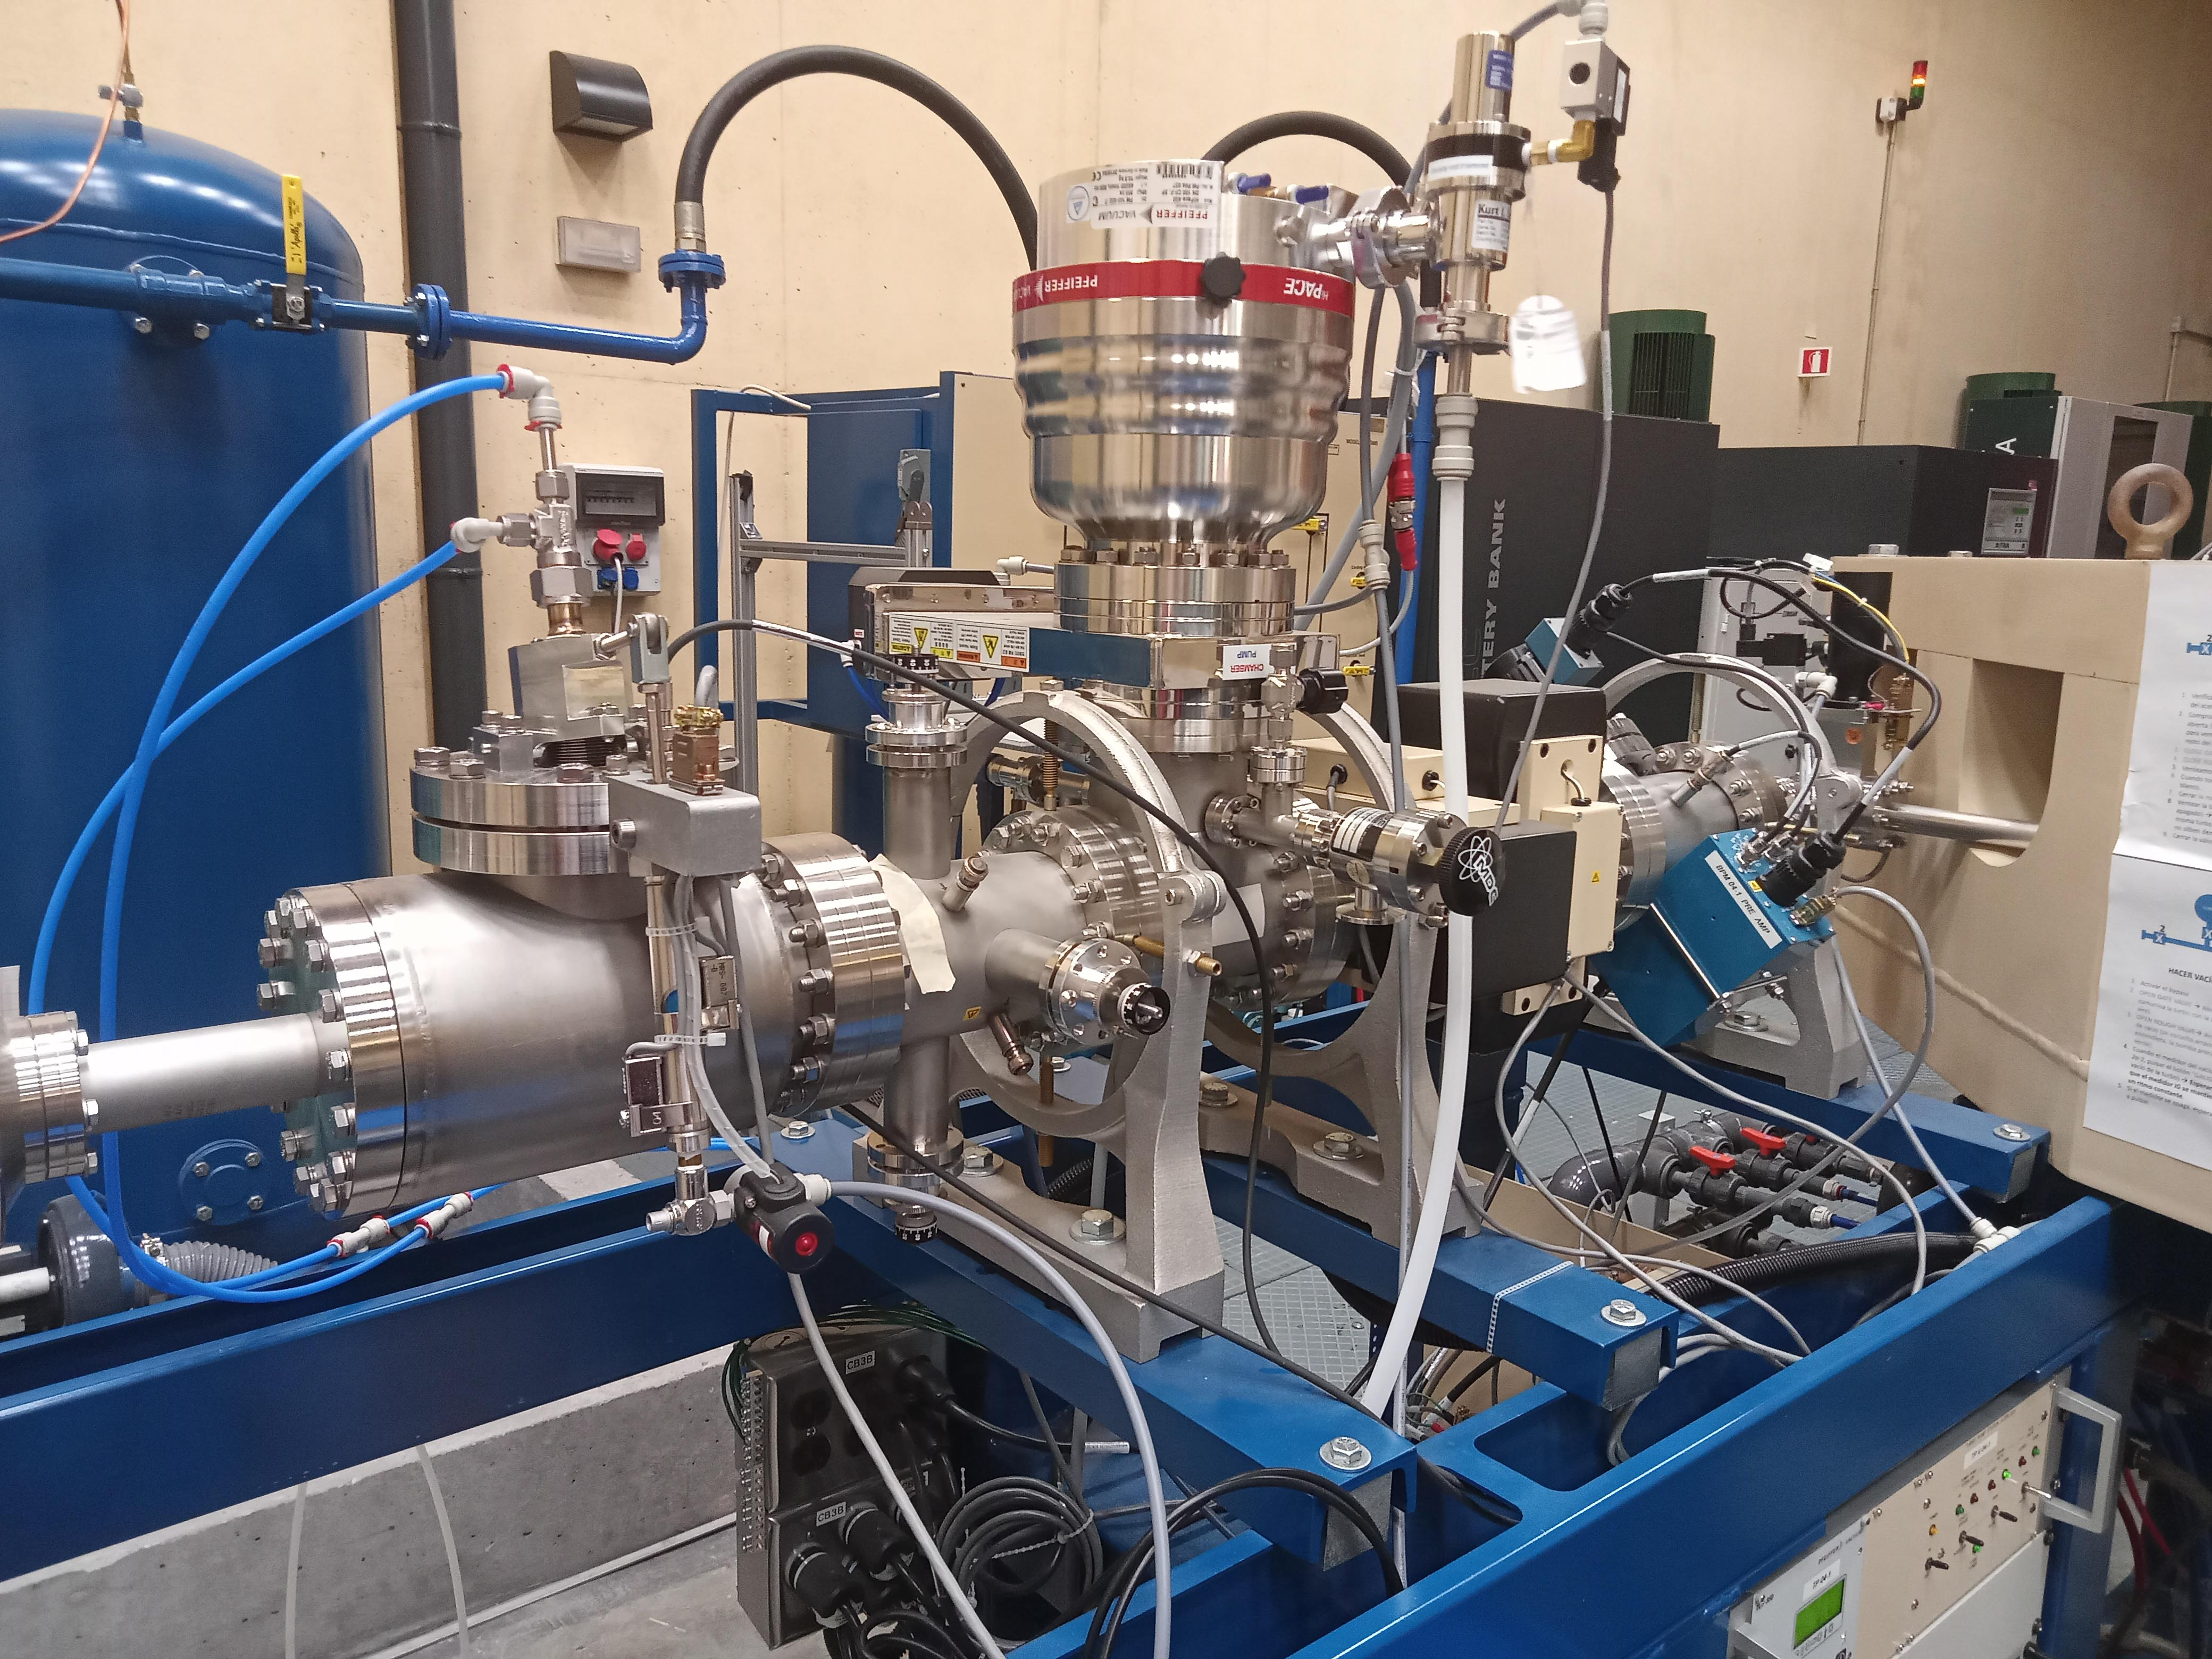
\includegraphics[width=0.50\textwidth]{neutronline_foto.jpg}
		\caption{Neutron line HiSPANoS.}
		\label{}
	\end{figure}
\end{frame}

\begin{frame}{Experimental setup}
	\begin{figure}[H]
		\centering
		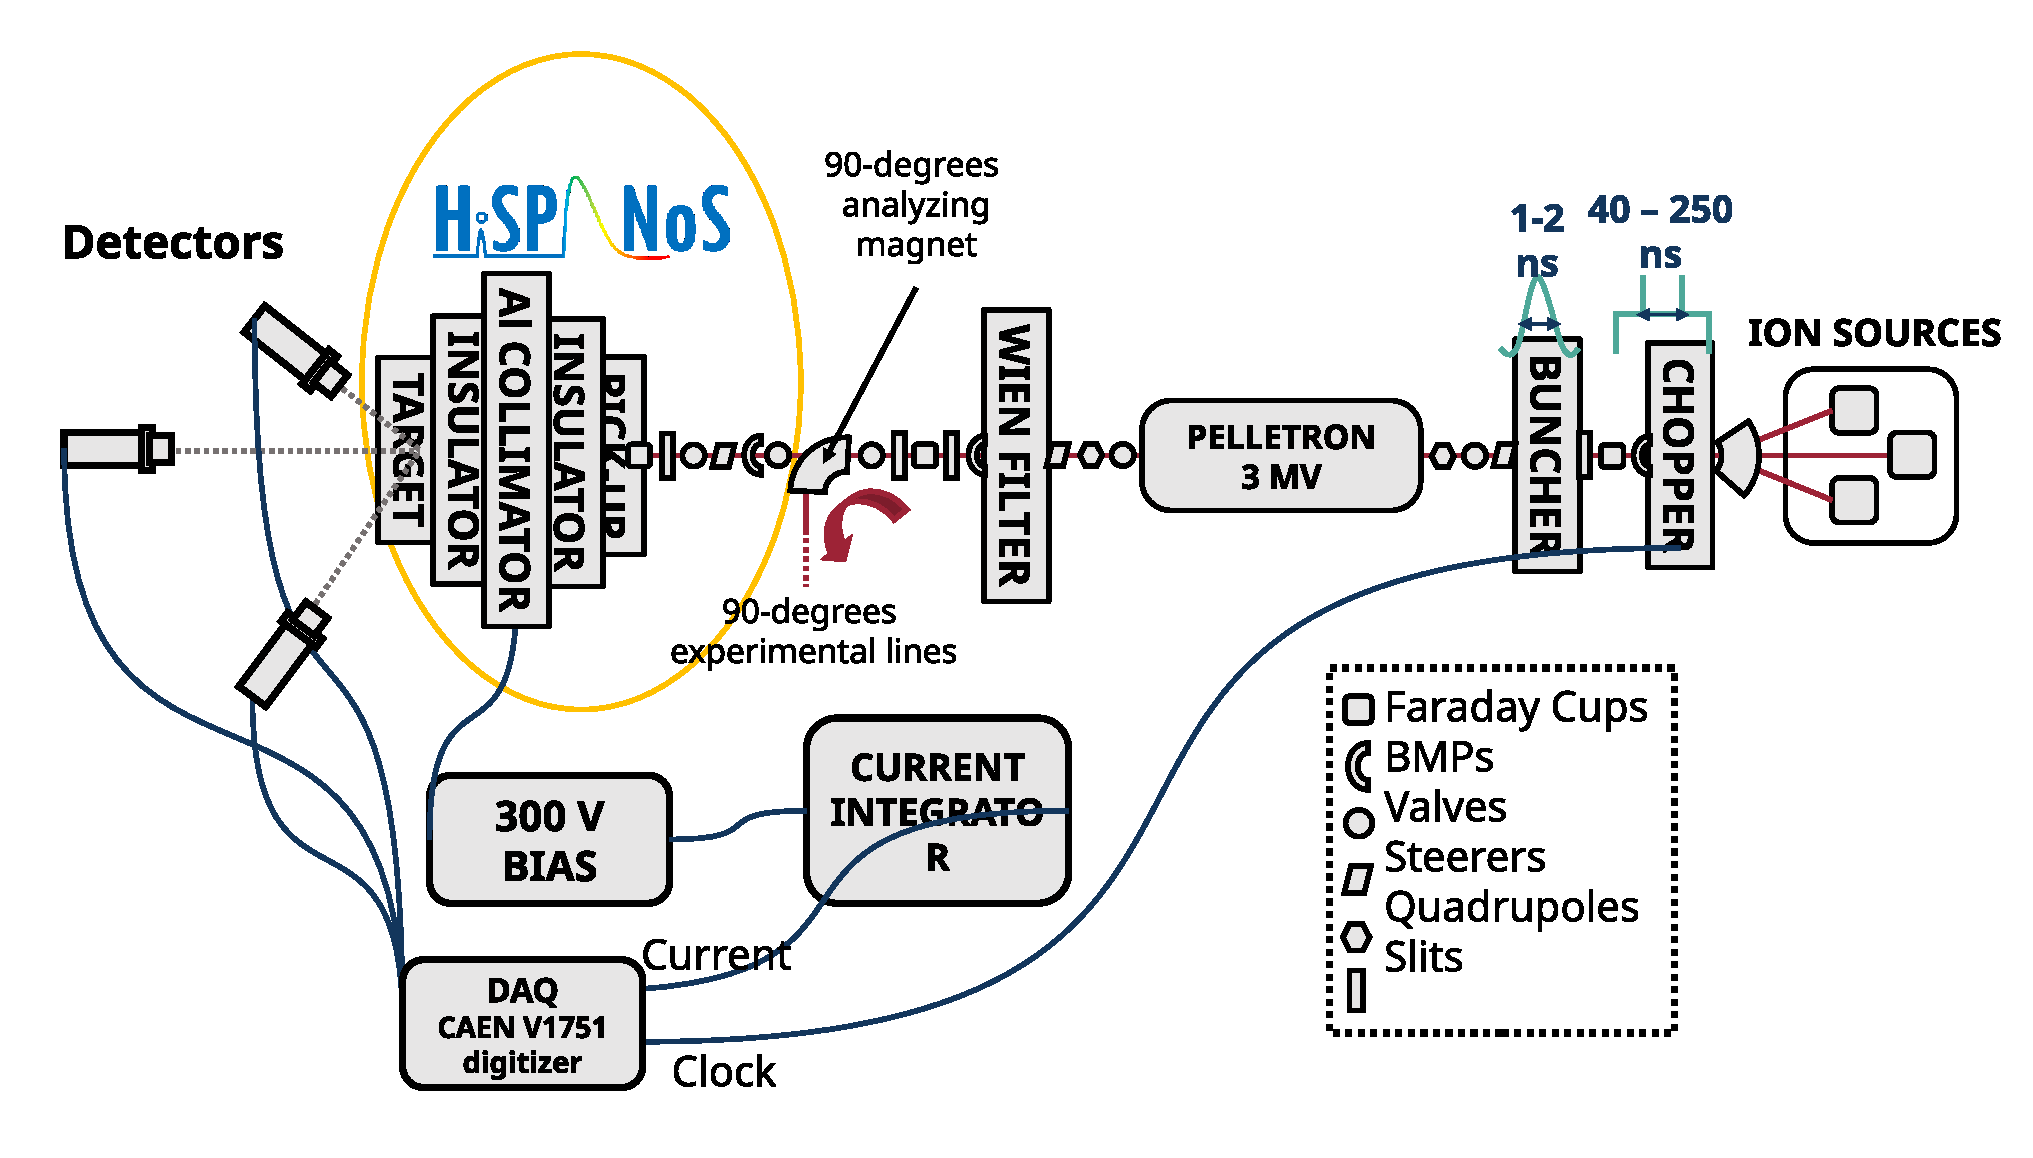
\includegraphics[width=0.80\textwidth]{tandemdiagrama.eps}
		\caption{Diagram of the CNA's Tandem accelerator}
		\label{}
	\end{figure}
	\begin{itemize}
		\item For $\alpha$, max energy of \qty{9}{\MeV}
		\item \textit{Buncher} not designed for $\alpha$ particles
	\end{itemize}
\end{frame}

\begin{frame}{Experimental setup: PSD}
	\begin{figure}[H]
		\centering
		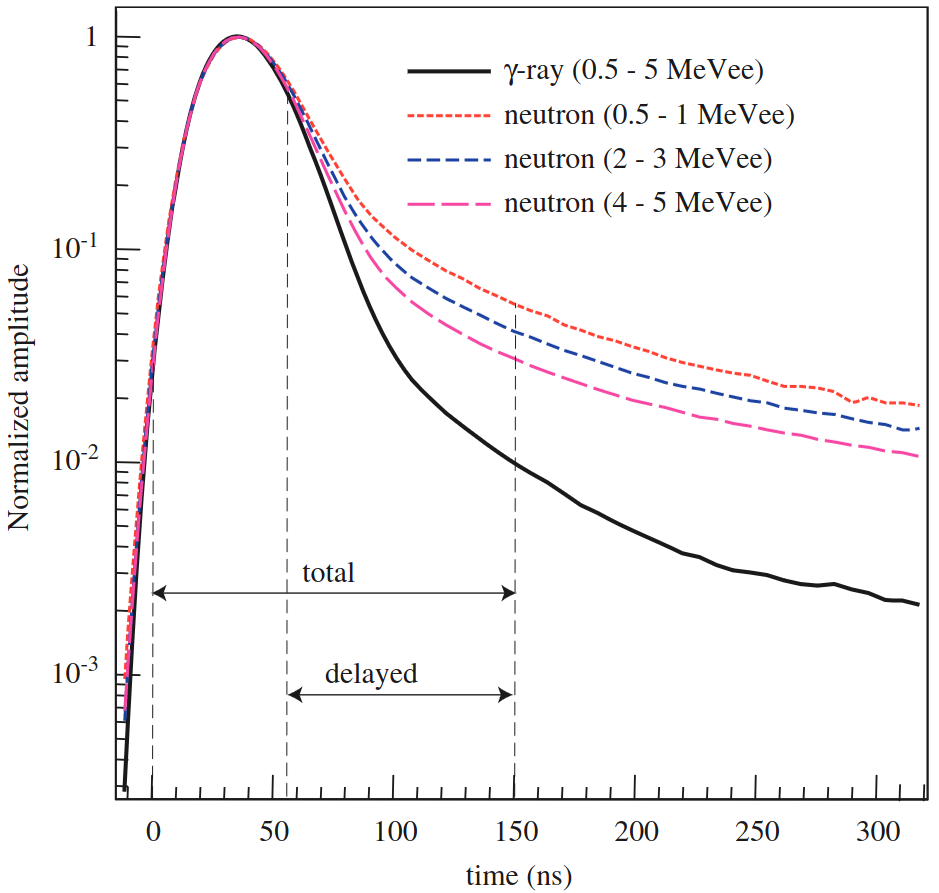
\includegraphics[width=0.45\textwidth]{psd_explanation.png}
		\caption{Pulses generated by different types of radiation. Figure from C. Guerrero et al. \cite{guerrero2008}.}
		\label{}
	\end{figure}
	\begin{equation}
		\text{PSD} = \frac{\text{delayed}}{\text{fast}+\text{delayed}}
	\end{equation}
\end{frame}

\begin{frame}{Experimental setup: PSD}
	\begin{figure}[H]
		\centering
		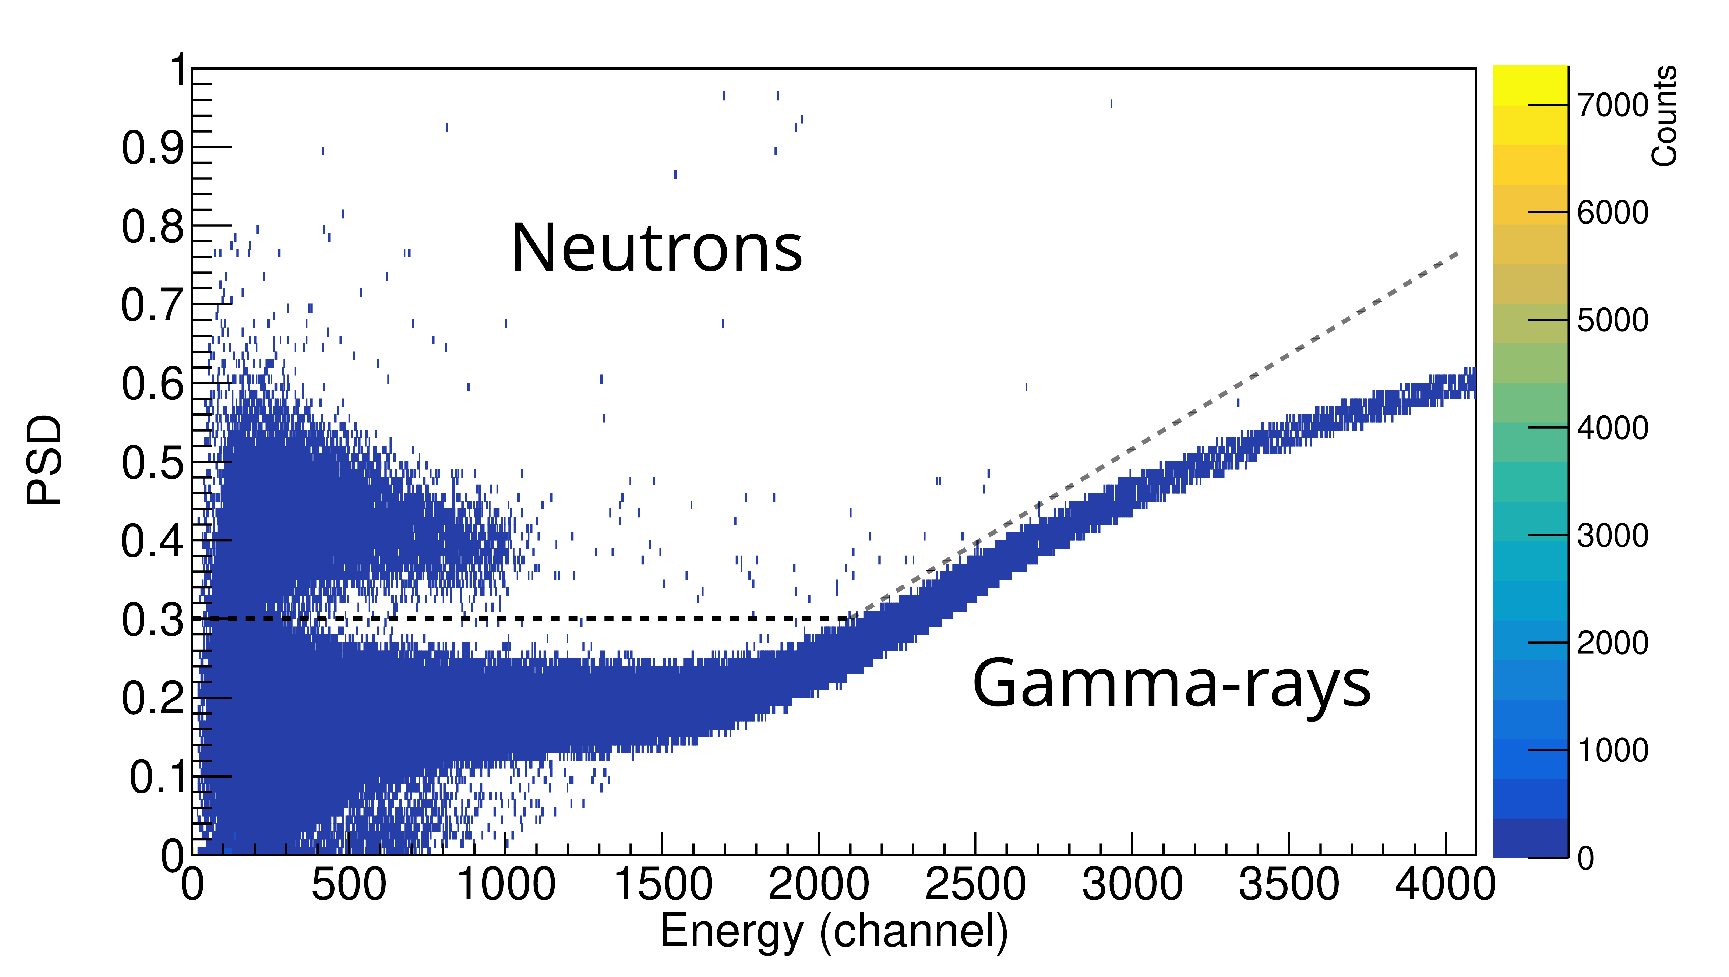
\includegraphics[width=0.85\textwidth]{example_psd.eps}
		\caption{Separation of neutrons and $\gamma$-rays by PSD of a MONSTER measurement.}
		\label{}
	\end{figure}
\end{frame}



%	ACTIVACION



\begin{frame}{Measurement of TTY by activation}
	\[ \text{\Aliso} + \alpha \longrightarrow \text{\Piso} + \text{n}   \]
	\centering
	$t_{1/2} = \qty{2.498(4)}{\minute}$; 
	$I_{511} = \num{1.99710(8)}$
	\begin{figure}[H]
		\centering
		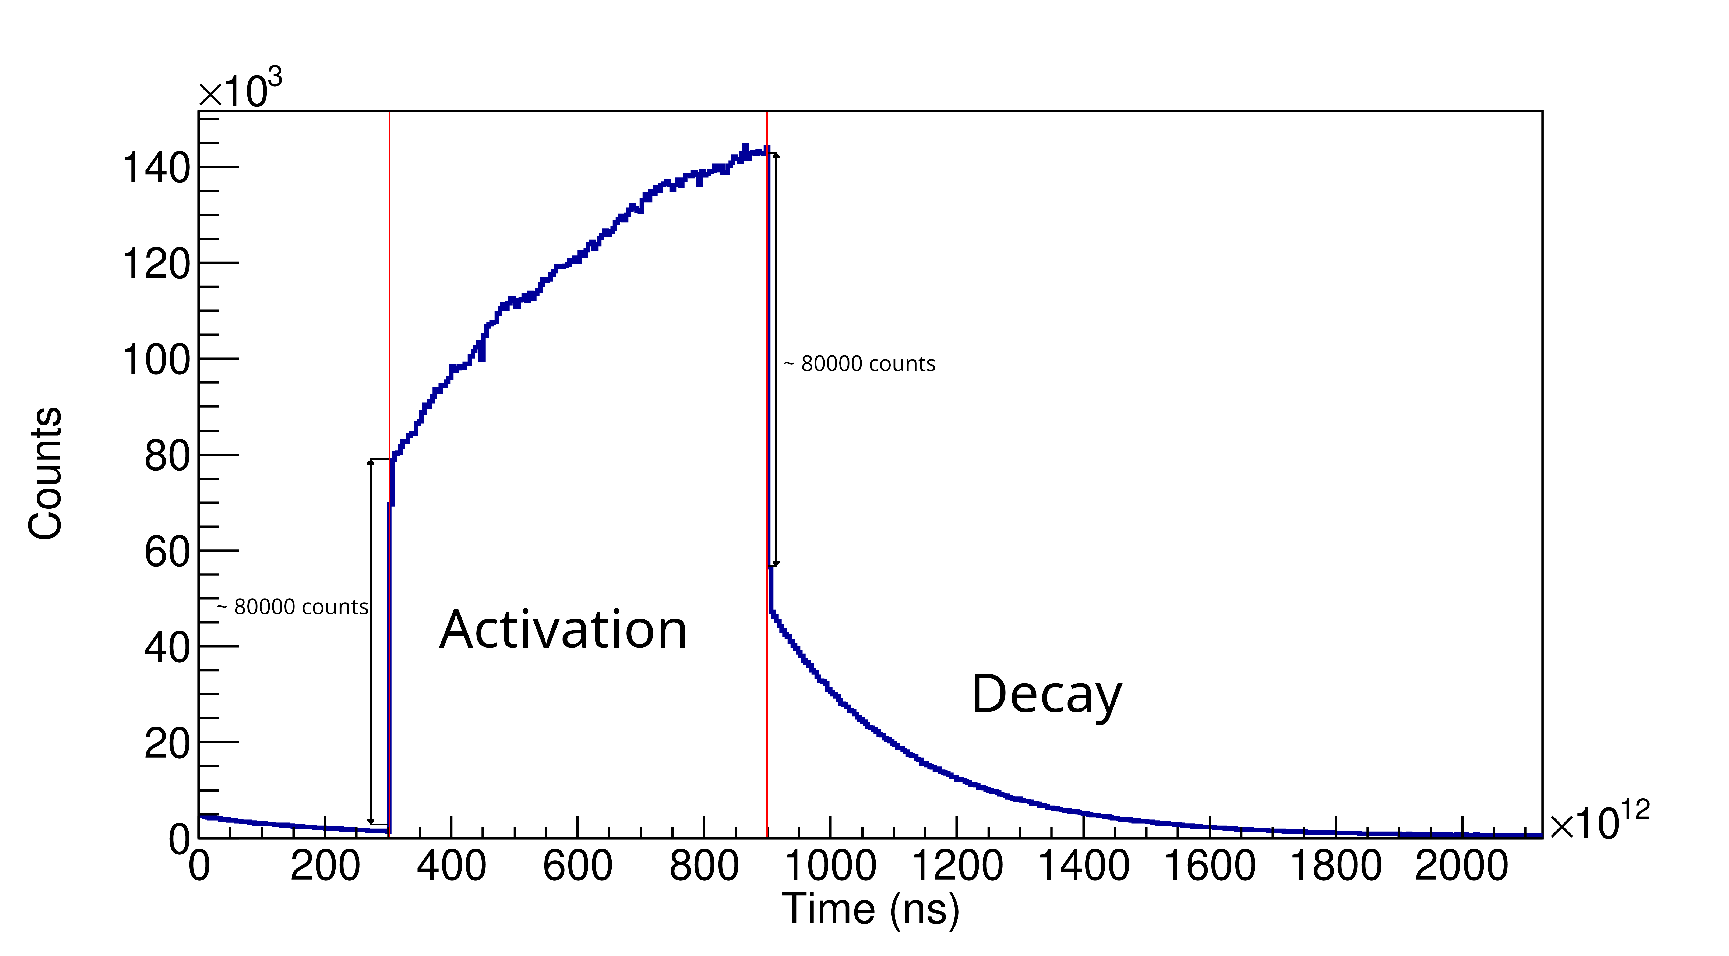
\includegraphics[width=0.80\textwidth]{example_activation_time_histogram.eps}
		\caption{Histogram of LaBr\textsubscript{3} detector counts against time.}
		\label{example_activation_time_histogram}
	\end{figure}
\end{frame}

\begin{frame}{Measurement of TTY by activation: analysis}
	Number of \Piso nuclei:
	\begin{equation}
		\ddt{N(t)} = P(t) -\lambda N(t) = P(t) - A(t)
		\label{general_diffeq}
	\end{equation}

	Thick Target Yield definition:
	\begin{equation}
		\text{TTY} = \frac{P(t)}{I_\alpha(t)}
	\end{equation}

	Relationship between activation and counts:
	\begin{equation}
		A(t) = \frac{c(t) - b(t)}{I_{511} b_{\Delta t} \varepsilon_{511}}
	\end{equation}
\end{frame}

\begin{frame}{Measurement of TTY by activation: \textit{decay} analysis}
	Assuming constant current:
	\begin{equation}
		\ddt{N} = P -\lambda N
	\end{equation}

	Solution:
	\begin{equation}
		N(t) = \frac{P}{\lambda} + \left(  N_0 - \frac{P}{\lambda}  \right) e^{-\lambda t}
	\end{equation}

	After an irradiation of duration $\Delta t$:
	\[ N\textsubscript{EOA} =N(\Delta t) = \frac{P}{\lambda} \left(1 - e^{-\lambda \Delta t} \right)\Longrightarrow A\textsubscript{EOA}=P\left(1-e^{-\lambda\Delta t}\right)\Longrightarrow \]
	\begin{equation}
		P = \frac{A\textsubscript{EOA}}{1 - e^{-\lambda \Delta t}}
	\end{equation}
\end{frame}

\begin{frame}{Measurement of TTY by activation: \textit{decay} analysis}
	\begin{equation}
		\text{TTY} = \frac{P}{I_\alpha} = \frac{A_\text{EOA}}{I_\alpha \left( 1-e^{-\lambda \Delta t}  \right)} = 
		\frac{c_\text{EOA}}{I_\alpha \left( 1-e^{-\lambda \Delta t}  \right) I_{511} b_{\Delta t} \varepsilon_{511}  }
	\end{equation}
	\begin{columns}
	\column{0.65\textwidth}
	\begin{figure}[H]
		\centering
		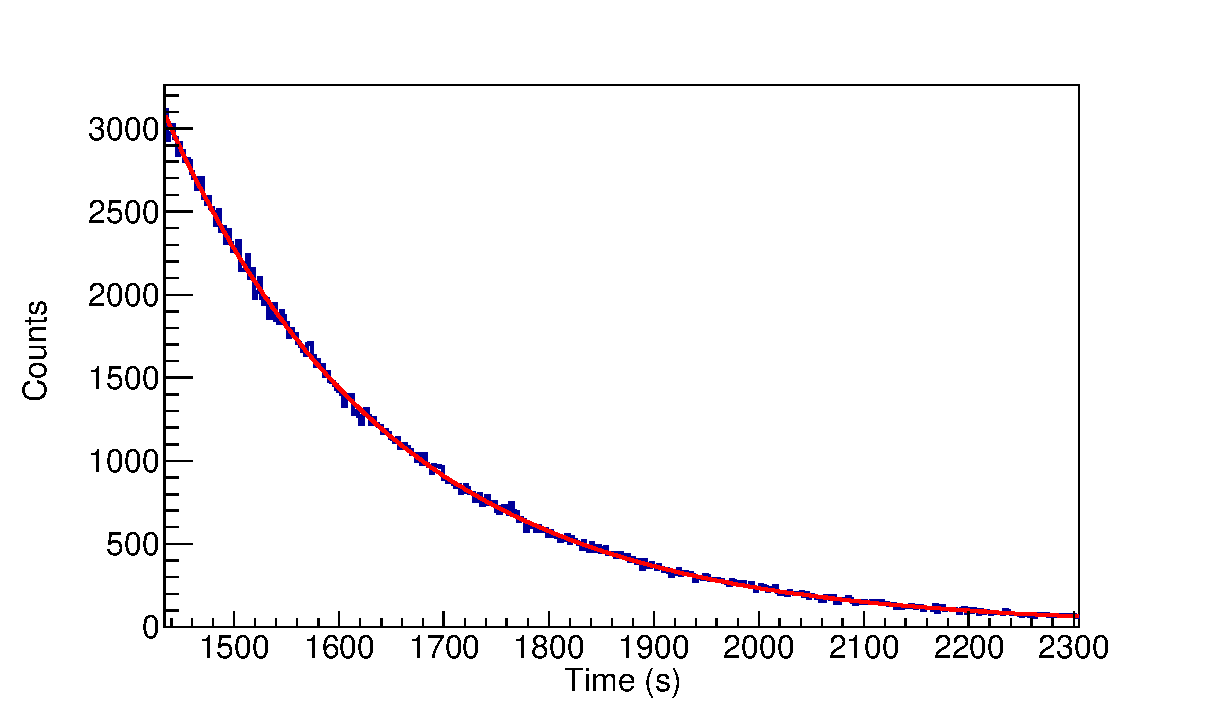
\includegraphics[width=\textwidth]{example_decay_fit.eps}
		\caption{Decay fit.}
		\label{decay_fit}
	\end{figure}
	\column{0.35\textwidth}
	Fit to exponential decay law plus a background:
	\begin{equation}
		c(t) = c_\text{EOA} e^{-\lambda t} + B
	\end{equation}
	\begin{itemize}
		\item Simple, fast
		\item Standard
		\item Assumes constant current
	\end{itemize}
	\end{columns}
\end{frame}

\begin{frame}{Measurement of TTY by activation: results}
	\begin{figure}[H]
		\centering
		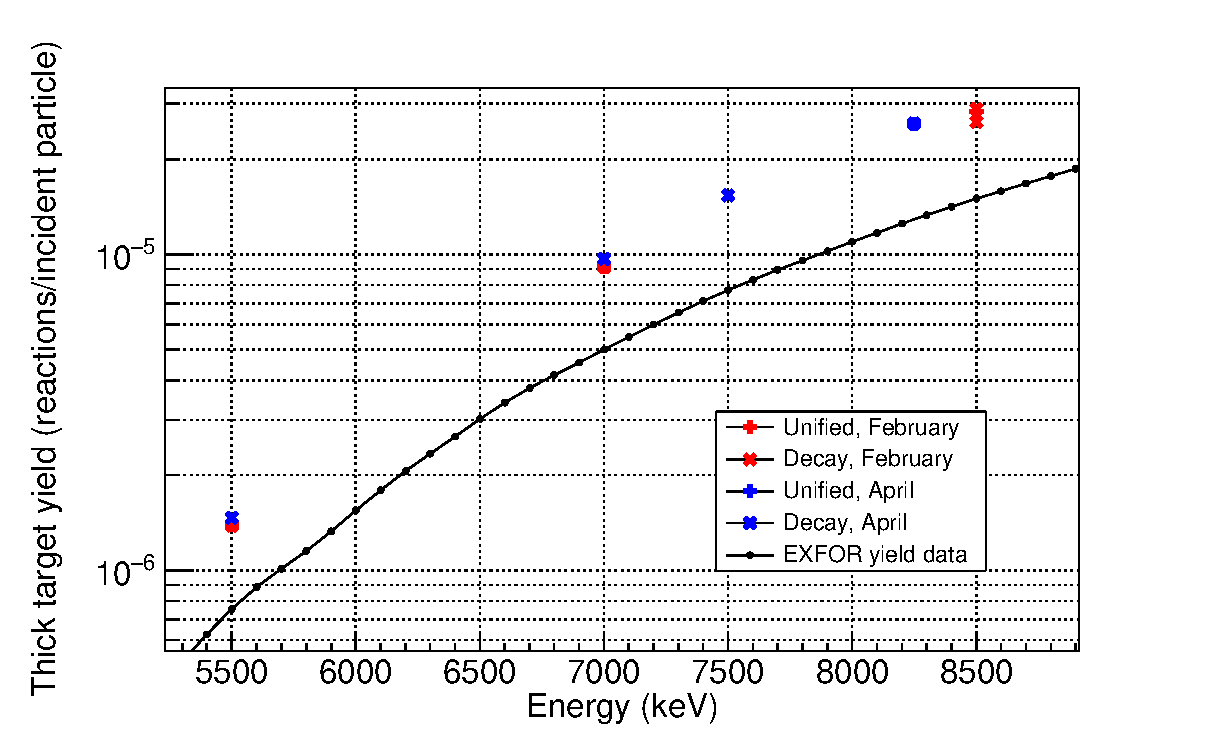
\includegraphics[width=0.80\textwidth]{activation_final_results.eps}
		\caption{Results obtained along with those from G. J. H. Jacobs and H. Liskien \cite{jacobs} and a version scaled by \num{1.9}.}
		\label{activation_final_results}
	\end{figure}
	Great systematic error, but same shape of TTY against energy.
\end{frame}




%	PULSADO



\begin{frame}{Energy spectra by ToF: Principle}
	\begin{itemize}
		\item Pulsed beam
		\item \textit{Gamma flash} $L/c$ time later
		\item Neutron response with energies:
	\end{itemize}
	\begin{equation}
		E_n=\frac{1}{2} m_n \left( \frac{L}{\text{ToF}} \right)^2 = \frac{1}{2} m_n \left( \frac{L}{t_n - t_{flash} + L/c} \right)^2
	\end{equation}
	\begin{figure}[H]
		\centering
		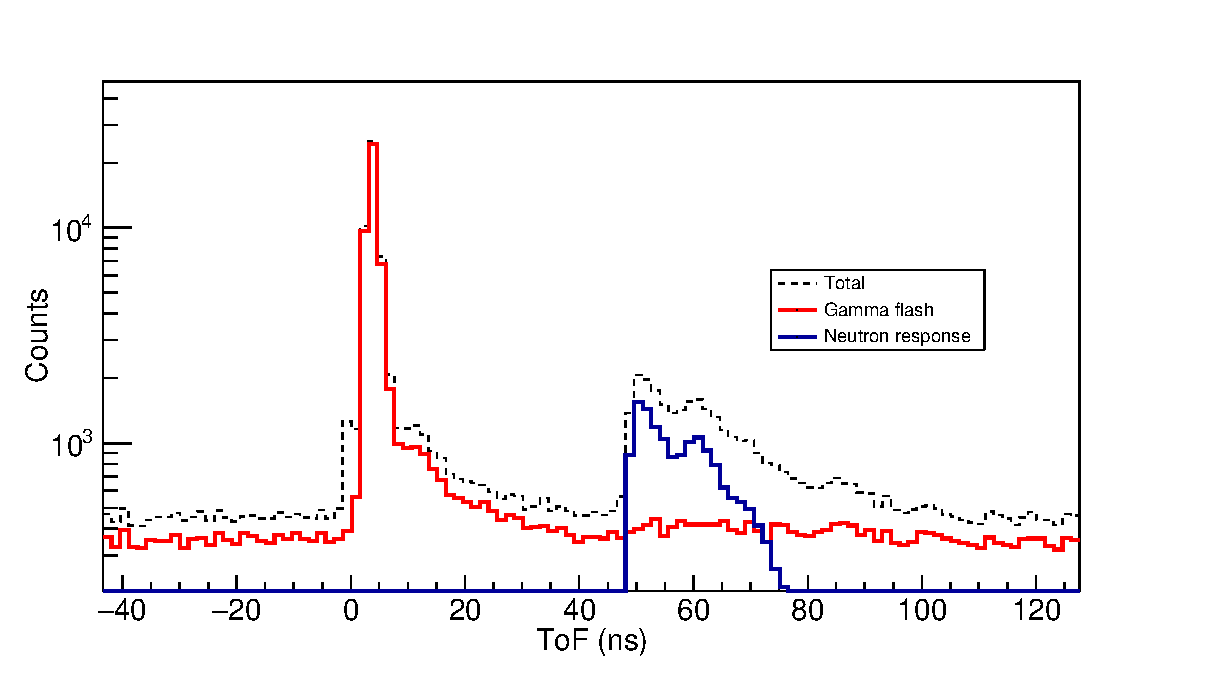
\includegraphics[width=0.70\textwidth]{separated_tof.eps}
		\caption{ToF of a measurement: \textit{gamma flash} and neutron response.}
		\label{separated_tof}
	\end{figure}
\end{frame}

\begin{frame}{Energy spectra by ToF: Simple analysis}
	\[E_n=\frac{1}{2} m_n \left( \frac{L}{\text{ToF}} \right)^2 = \frac{1}{2} m_n \left( \frac{L}{t_n - t_{flash} + L/c} \right)^2\]
	\begin{itemize}
		\item Correct by efficiency
		\item Present results per $\alpha$, solid angle and energy
	\end{itemize}
	\begin{figure}[H]
		\centering
		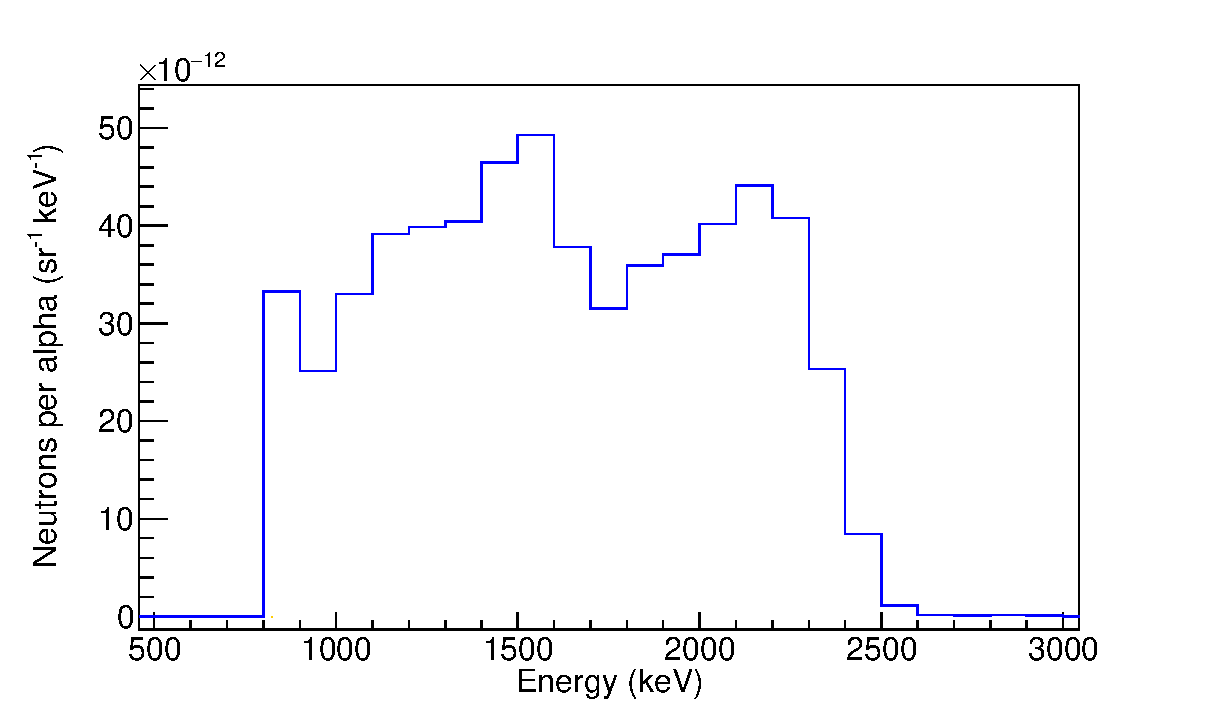
\includegraphics[width=0.60\textwidth]{pulsed_energysimple.eps}
		\caption{Energy spectra for measurement 2.}
		\label{}
	\end{figure}
\end{frame}

\begin{frame}{Energy spectra by ToF: Deconvolution analysis}
	\begin{figure}[H]
		\centering
		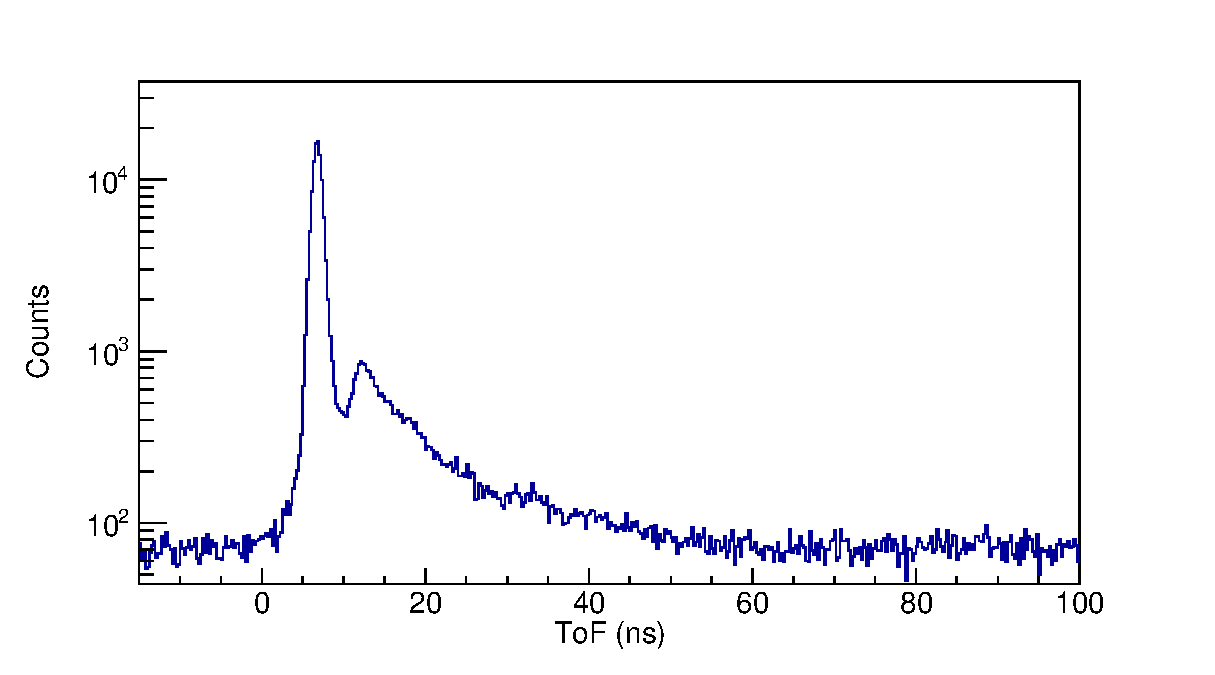
\includegraphics[width=0.95\textwidth]{uneven_gflash.eps}
		\caption{\textit{Gamma flash} for measurement 5.}
		\label{uneven_gflash}
	\end{figure}
\end{frame}

\begin{frame}{Energy spectra by ToF: Deconvolution analysis}
	\begin{figure}[H]
		\centering
		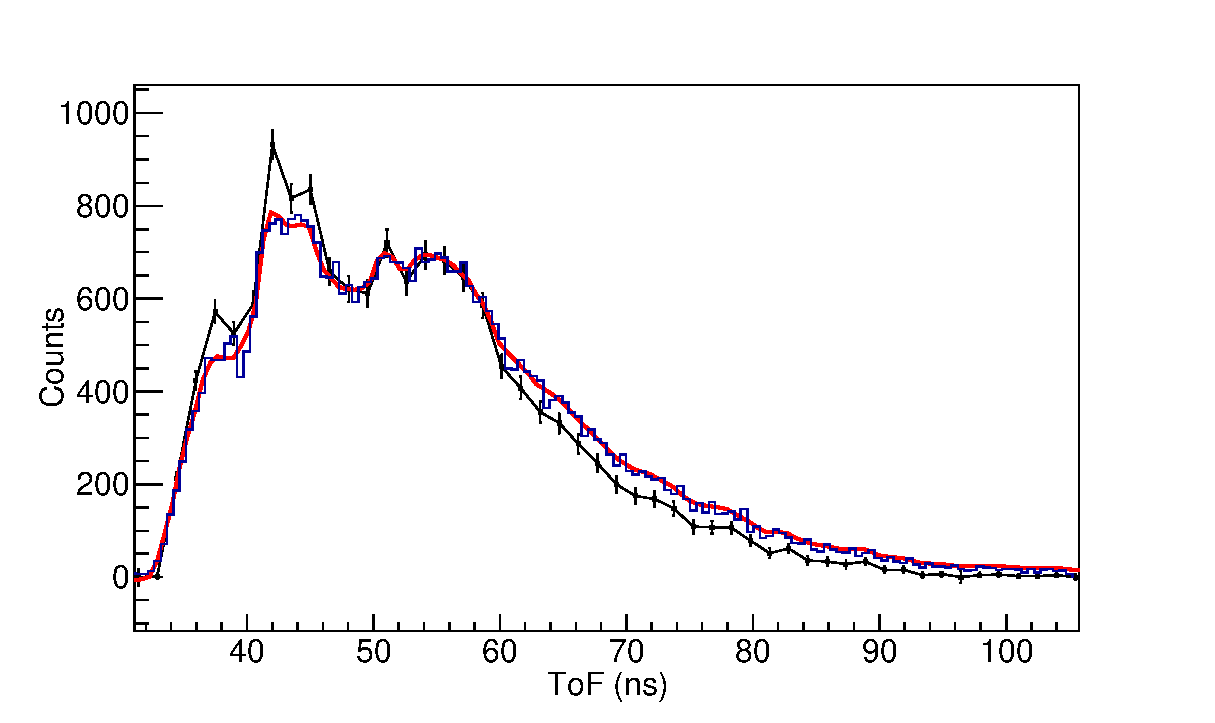
\includegraphics[width=0.70\textwidth]{pulsed_deconvolution_delta.eps}
		\caption{Deconvolution for measurement 2.}
		\label{}
	\end{figure}
	\begin{itemize}
		\item 50 parameters represent the spectrum in ToF
		\item Function uses the $\gamma$-flash to calculate the neutron response
		\item Result takes into account the shape of the $\alpha$ pulse
	\end{itemize}
\end{frame}

\begin{frame}{Energy spectra by ToF: Results}
	\begin{figure}[H]
		\centering
		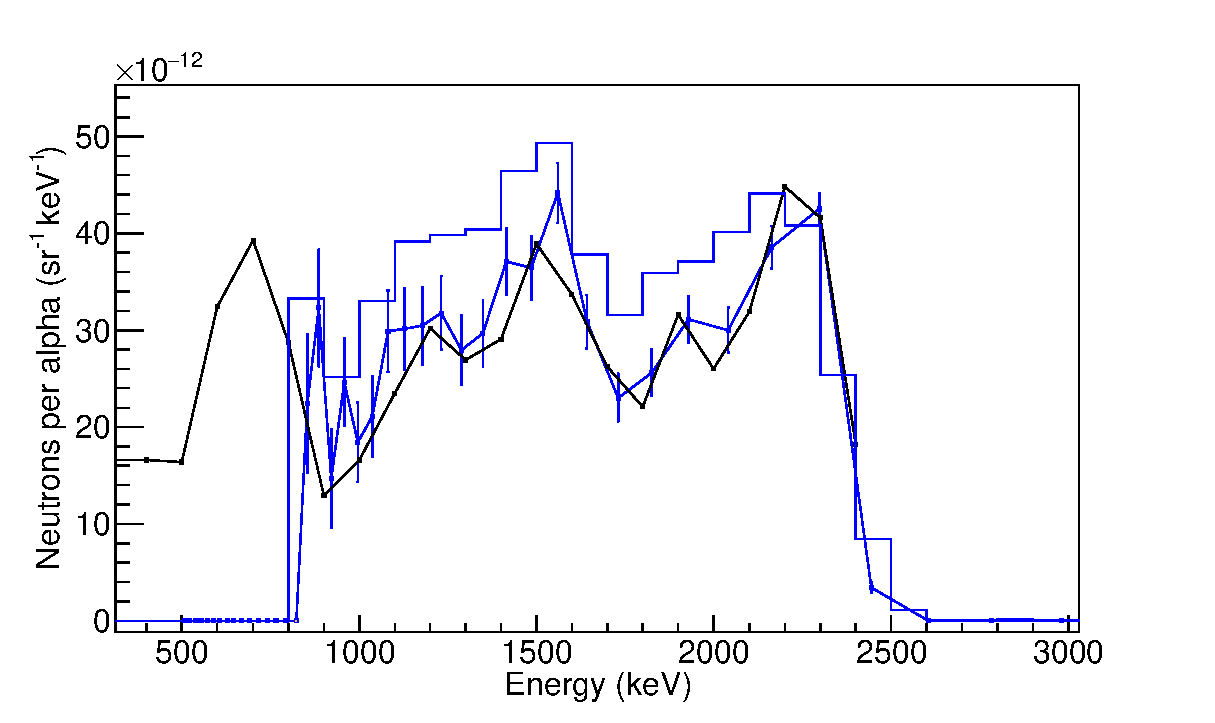
\includegraphics[width=0.70\textwidth]{pulsed_5mev.eps}
		\caption{Results for \qty{5.5}{\MeV}, along with G. J. H. Jacobs and H. Liskien\cite{jacobs}.}
		\label{}
	\end{figure}
	\begin{itemize}
		\item Deconvolution shifts counts from low to high energies
		\item Little or no improvement to energy resolution
		\item Simple method overestimates, specially for low energies
	\end{itemize}
\end{frame}

\begin{frame}{Energy spectra by ToF: Results}
	\begin{figure}[H]
		\centering
		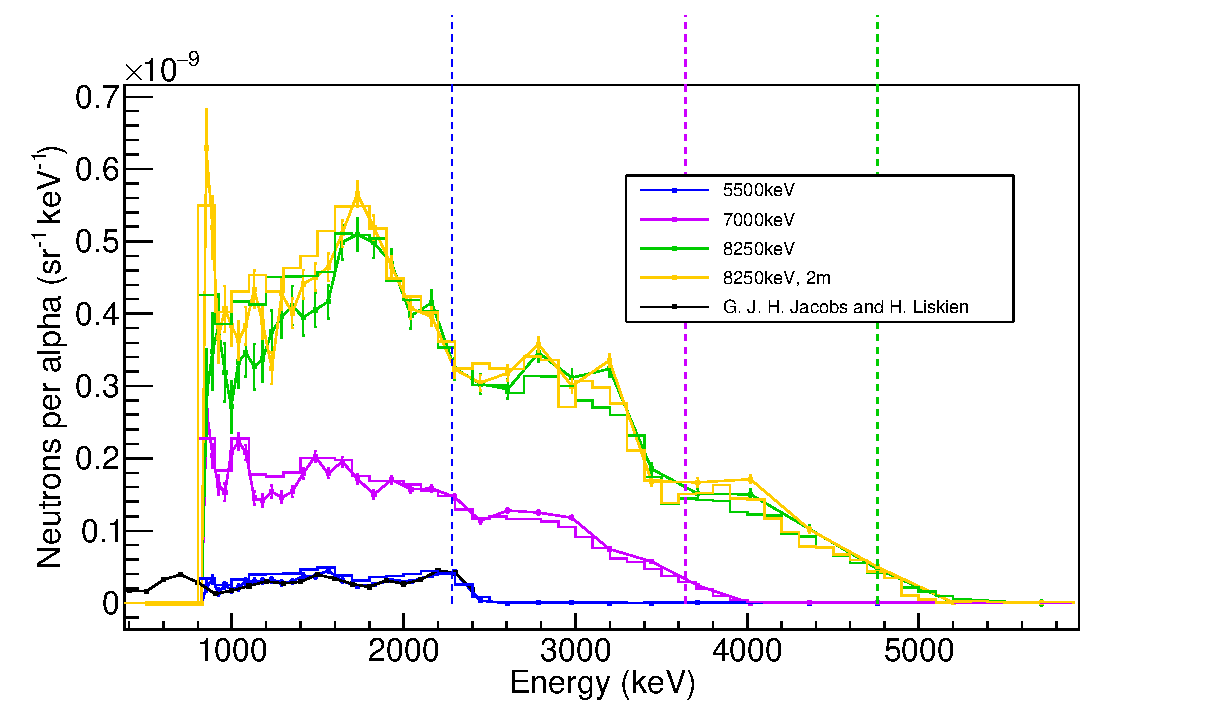
\includegraphics[width=0.95\textwidth]{pulsed_results.eps}
		\caption{All results, simple and deconvolution}
		\label{}
	\end{figure}
\end{frame}

\begin{frame}{Conclusions}
	\begin{itemize}
		\item TTY: agreement between measurements, but big systematic error
		\item Energy spectra: good agreement when using a simple deconvolution
		\item CNA/HiSPANoS capable of reasonably good activation and pulsed beam measurements
	\end{itemize}
\end{frame}

\begin{frame}{References}
\begin{thebibliography}{5}
	\bibitem{jacobs}G. J. H. Jacobs and H. Liskien, Energy Spectra of Neutrons produced by $\alpha$ particles in thick targets of light elements, Annals of Nuclear Energy 10, 541 (1983)
%	\bibitem{hispanos}B. Fernández et al.,HiSPANoS facility and the new neutron beam line for TOF measurements at the Spanish National Accelerator Lab (CNA), 2020 J. Phys.: Conf. Ser. 1643 012033
	\bibitem{guerrero2008}C. Guerrero et al., Analysis of the BC501A neutron detector signals using the true pulse shape, Nuclear Instruments and Methods in Physics Research A 597 (2008) 212–218
%	\bibitem{astro1}F. Käppeler et al., The \textit{s} process: Nuclear physics, stellar models, and observations, Rev. Mod. Phys. 83, 157 – 193 (2011)
%	\bibitem{astro2}J. Pereira and F. Montes, Theoretical uncertainty of \an reactions relevant for the nucleosynthesis of light r-process nuclei in neutrino-driven winds, Phys. Rev. C 93, 034611 (2016)
%	\bibitem{neutron_in_an}NV.A. Kudryavtsev, P. Zakhary. B. Easeman, Neutron production in \an reactions, Nucl. Instrum. Methods Phys. Res. A 972 (2020)
%	\bibitem{MANY}N. Mont-Geli et al., miniBELEN: A modular neutron counter for \an reactions, EPJ Web of Conf., 284 (2023) 06004
	\bibitem{nucleardatasheets}M. Shamsuzzoha Basunia, Nuclear Data Sheets 111, 2331 (2010)
	\bibitem{INDC}S. S. Westerdale et al., (alpha,n) Nuclear Data Evaluations and Data Needs, Technical Report, INDC(NDS)-0836 (2022)
	\bibitem{CNA}Gómez-Camacho, J., García López, J., Guerrero, C. et al., Research facilities and highlights at the Centro Nacional de Aceleradores (CNA). Eur. Phys. J. Plus 136, 273 (2021)
%	\bibitem{labr}Alain Iltis et al., Lanthanum halide scintillators: Properties and applications, Nuclear Instruments and Methods in Physics Research Section A: Accelerators, Spectrometers, Detectors and Associated Equipment, Volume 563, Issue 2 (2006)
%	\bibitem{MONSTER}A R Garcia et al., MONSTER: a time of flight spectrometer for $\beta$-delayed neutron emission measurements, 2012 JINST 7 C05012
%	\bibitem{ej301}NEUTRON/GAMMA PSD EJ-301, EJ-309
%	\bibitem{jacobssupport1}R. Heaton et al., Neutron production from thick-target \an reactions, Nuclear Instruments and Methods A 276, 529 (1989)
%	\bibitem{jacobssupport2}J. K. Bair and J. Gomez del Campo, Neutron Yields from Alpha-Particle Bombardment, Nuclear Science and Engineering 71, 18 (1979)
%	\bibitem{CAEN}CAEN 751 Waveform Digitizer Family, CAEN SpA
%	\bibitem{ROOT}Rene Brun and Fons Rademakers, ROOT - An Object Oriented Data Analysis Framework, Proceedings AIHENP'96 Workshop, Lausanne, Sep. 1996, Nucl. Inst. \& Meth. in Phys. Res. A 389 (1997) 81-86. See also "ROOT" [software], Release 6.28/04
%	\bibitem{angeant4}E. Mendoza et al., Neutron production induced by $\alpha$-decay with Geant4, Nuclear Inst. and Methods in Physics Research, A 960 (2020) 163659
\end{thebibliography}
\end{frame}

\end{document}
